\section{Evolutionary Analysis}

We performed experiments to characterize the evolution of tag-mediated connectivity networks under our five tag-matching metrics.
Our experiments compared scenarios with selection for more-constrained networks, where individual tags needed to ensure simultaneously tight affinity with several other tags, and scenarios with selection for less-constrained networks, where individual tags only needed to ensure tight affinity with one other tag. 
First, we evolved sets of tags to match explicitly specified graphs, which allowed us to directly control the level of network constraint selected for.
Second, we evolved full-fledged SignalGP programs that use tag matching to control module activation.
In these experiments, we indirectly controlled selection for network constraint by comparing a two diagnostic problems.
In the first, the changing-signal task, programs with sparse interactions between modules are known to evolve.
In the second, the directional-signal task, programs with dense interactions between modules are known to evolve.
SignalGP experiments also allowed us to investigate if tag-matching metrics exhibited different performance characteristics in a more generalized, complex domain.

\subsection{Graph Matching Task}

\begin{figure*}

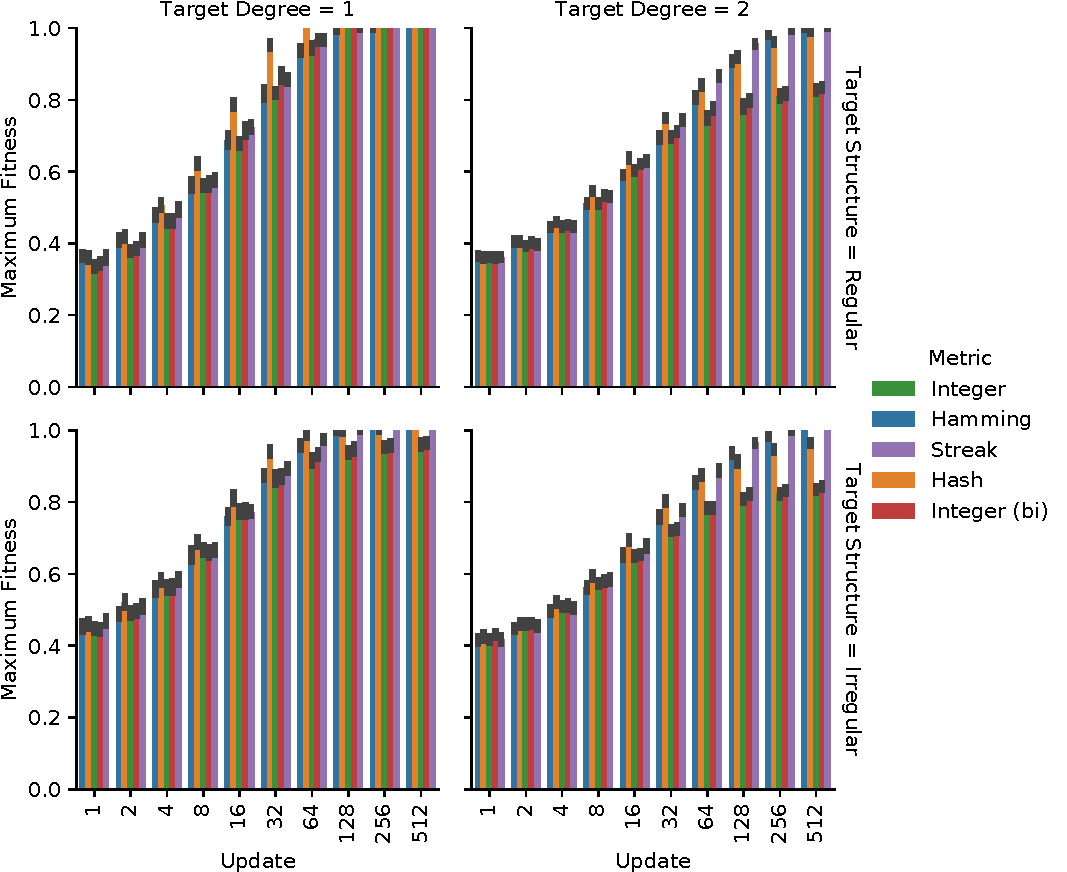
\includegraphics[width=\linewidth]{img/target_evolve/viz=max-fitness-bar+_data_hathash_hash=673d309ab90e91d1+_script_fullcat_hash=6c7848b1ac357236+ext=}

\caption{
Trajectories of adaptive evolution for each tag-matching metric on the 64-node graph-matching task.
Maximum fitness represents the best fitness value for any individual within a population.
Here report using each metric's best-performing per-bit mutation rate.
(See Supplementary Figure \ref{fig:evolve_mutsweep} for survey showing how mutation rate affects adaptive evolution under each metric.)
Note log-scale x-axes.
Shaded area represents bootstrapped 95\% confidence intervals across 20 replicate observations.
}
\label{fig:evolve_bests}
\end{figure*}


In this evolutionary experiment, we evolved genomes consisting of 32 bitstring tags to establish a pattern of connectivity mirroring that of a randomly-generated target bipartite graph.
Each bitstring tag in a genome corresponded to a node in the target graph.
Half of the graph nodes, comprising one partition of the graph, were designated as queries.
The other half of the graph nodes, comprising the other partition of the graph, were designated as operands.
To evaluate the fitness of a genome, we harvested its operand tags placed them into a tag-matching data structure.
This data structure allowed us to determine the best matches among the set of operand tags for each query tag (the operand tags with minimal match distance to that query).
For each query tag, we recorded as many best-match results as outgoing connections from the corresponding node in the target graph.
Fitness was calculated as the fraction of best-match query and operand tag pairs that correctly corresponded to edges in the target graph.

We controlled the degree of tag-matching constraint imposed by the target graph by manipulating:
\begin{enumerate}
  \item the number of edges between queries and operands, and
  \item whether edges were assigned evenly such that all nodes had identical degree (regular structure) or were assigned at random, likely causing some nodes to have high degree (irregular structure).
\end{enumerate}
We tested target graphs mean degree 1 and 2 and both regular and irregular construction.
Regular, degree 1 graphs imposed the least tag-matching constraint.
Irregular, degree 2 graphs imposed the most tag-matching constraint.
\href{doi.org/10.17605/OSF.IO/GW5MC}{Supplementary Figure \ref{fig:graph_layouts}} shows examples of these graph layouts \cite{Moreno_Ofria_2020}.

For each target graph configuration, we surveyed each metric's performance over ten per-bit mutation rates ranging from 0.75 expected mutations per genome to 16.0 expected mutation rates per genome.
We then isolated each metric and target graph configuration combination's most favorable mutation rate as defined by sum population-maximum fitness across updates.
\footnote{
\href{doi.org/10.17605/OSF.IO/GW5MC}{Supplementary Figure \ref{fig:evolve_mutsweep}} summarizes evolutionary performance of metrics across mutation rate/target graph configurations \cite{Moreno_Ofria_2020}.
All metrics show evidence of a performance maxima within the range of mutation rates surveyed, except for the hash metric on the regular target graph of degree 1.
In this case, peak performance was observed on the lowest sampled mutation rate.
}

We ran 100 replicate 512-generation evolutionary runs for each mutation rate/target graph/metric combination.
We used a well-mixed population of size 500 and tournament selection with tournament size 7.

Figure \ref{fig:evolve_bests} plots population-maximum fitness over the course of evolutionary runs.
Surprisingly, the hash metric enables faster adaptive evolution than all other metrics toward matching the least-constrained target graph (non-overlapping 95\% CI).
On more-constrained target graphs with mean degree 2, the hash metric's advantage in rapid adaptive evolution disappears.
In fact, on the most-constrained target graph (irregular structure with mean degree 2) the hash metric yields significantly lower-quality solutions at the end of evolutionary runs than the streak and hamming metrics.

The integer and bidirectional integer metrics successfully evolve connectivity patterns matching the unconstrained target graph (regular structure with mean degree 1) but yield lower-quality solutions than other metrics on constrained target graphs (non-overlapping 95\% CI).

The streak metric facilitates slightly faster adaptive evolution than the hamming metric, especially on mean degree 2 regularly configured target graphs (non-overlapping 95\% CI).

We performed the same evolutionary experiment with 64-node target graphs and observed qualitatively similar results (\href{doi.org/10.17605/OSF.IO/GW5MC}{Supplementary Figures \ref{fig:evolve_bests64}, \ref{fig:evolve_big_mutsweep}} \cite{Moreno_Ofria_2020}).

\subsection{Changing-signal Task}

\begin{figure}[!htbp]
\centering
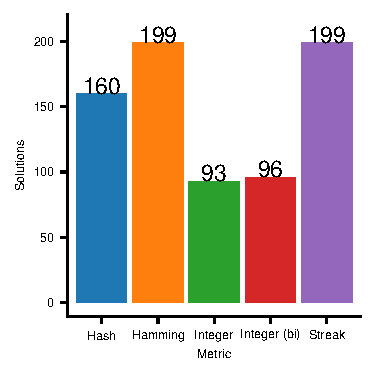
\includegraphics[width=0.75\linewidth]{img/gp_results/panel-cst-sols.pdf}

\caption{
Evolutionary performance of tag-matching metrics on the changing signals task.
Shows the numbers of replicates out of 200 that produced a complete task solution to the changing-signal and directional-signal task respectively.
Results for each metrics' best-performing mutation rate are reported.
}

\label{fig:cst-sols}

\end{figure}


% % @AML: I don't like this heading. 
% \subsection{Evolving tag-based genetic programs}

% % -- Introduce SignalGP --
The SignalGP genetic programming representation employs tag-based referencing to facilitate event-driven program execution \citep{lalejini2018evolving}.
In SignalGP, programs are segmented into modules (functions) that may be automatically triggered by exogenously- or endogenously-generated signals.
Tags specify the relationship between signals and signal-handlers (program modules), triggering the module with the closest matching tag to run its linear sequence of instructions.
% SignalGP makes explicit the concept of signals (events), which comprise a tag and, optionally, signal-specific data.

The SignalGP instruction set, in addition to including traditional GP operations, allows programs to generate arbitrarily-tagged internal signals and broadcast arbitrarily-tagged external signals, and otherwise work in a tag-based context.
% Instructions contain arguments, including an evolvable tag, that may modify the instruction's effect, often specifying memory locations or fixed values.
% Instructions may refer to program modules using tag-based referencing; for example, an instruction may trigger the execution of a program module using the instruction's tag to specify which module to trigger.
SignalGP also supports genetic regulation with promoter and repressor instructions that, when executed, allow programs to adjust how well subsequent signals match with a target function (specified with tag-based referencing). % todo - cite regulation paper
% TODO - when reviews come back, cite regulation paper?
See \citep{lalejini2018evolving} for a more detailed description of SignalGP.

% -- Changing-signal task --

% \subsubsection{Solving a minimally constrained problem}

The changing-signal task requires SignalGP programs to express a distinct response to each of $K$ environmental signals, each designated with a unique tag.
Programs express a response by executing one of $K$ response instructions.
Successful programs can `hardcode' each response with the appropriate environmental signal, ensuring that each environmental signal's tag best matches the function containing the correct response.
Thus, SignalGP module tags are minimally constrained --- each needs to only match with a single environmental signal.

During evaluation, we afford programs 64 time steps to express the appropriate response after receiving a signal.
Once a program expresses a response or the allotted time expires, we reset the program's virtual hardware (resetting all executing threads and thread-local memory), and the environment produces the next signal.
Evaluation continues until the program correctly responds to each of the $K$ environmental signals or until the program expresses an incorrect response.
During each evaluation, programs experience environmental signals in a random order; thus, the correct \textit{order} of responses will vary and cannot be hardcoded.

% Experiment overview
% @AML: currently, this section outsources A LOT of the configuration details to the supplement. Need to discuss what level of detail we want to go into here.
% We compared the performance of SignalGP with each of the Hamming, Hash, Integer, Bidirectional Integer, and Streak tag-matching metrics.
For each tag-matching metric, we evolved 200 replicate populations (each with a unique random number seed) of 500 asexually reproducing programs in an eight-signal environment ($K=8$) for 100 generations.
We identified the most performant per-bit tag mutation rates (from a range of possible mutation rates) for each metric on the changing-signal task: 0.01 for the hamming and streak metrics, 0.002 for the hash metric, and 0.02 for the integer and bidirectional integer metrics.
%(these data are available in supplemental material \cite{Moreno_Ofria_2020})
Aside from tag mutation rate, the overall configuration used for each metric was identical.
We limited tag variation in offspring to tag mutation operators (bit flips) by initializing populations with a common ancestor program in which all tags were identical and by disallowing mutations that would insert instructions with random tags.
Our supplemental material gives the full configuration details for this experiment, including a guide for replication \cite{Moreno_Ofria_2020}.

% \begin{figure*}
  \begin{center}

  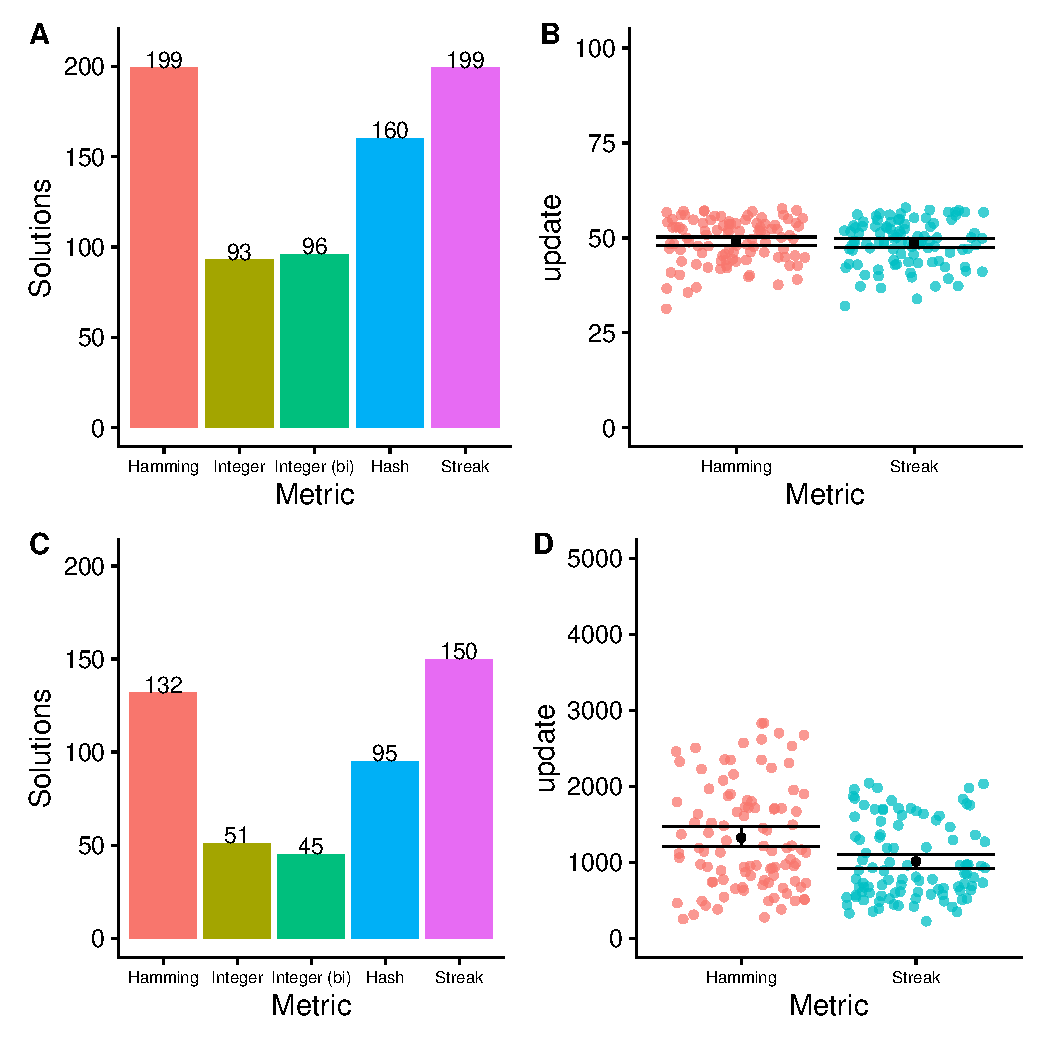
\includegraphics[width=\columnwidth]{img/gp_results/gp_results_panel}
  \caption{
  Todo - caption. A, B are changing-signal task; C, D are directional signal task.
  }
  \label{fig:gp_results}

  \end{center}
  \end{figure*}

Figure \ref{fig:cst-sols} gives the number of replicates that produced a successful SignalGP program (\textit{i.e.}, capable of achieving maximum fitness) for each tag-matching metric on the changing-signal task.
We compared the number of successful replicates across metrics using a pairwise Fisher's exact test with a Holm correction for multiple comparisons.

The hamming and streak metrics performed significantly better than all other metrics ($p < 5\times10^{-11}$); however, there was no significant difference in performance between the hamming and streak metrics.
To assess whether the streak metric produced solutions in fewer generations than the hamming metric, we ran 200 new replicates of each condition until 100 replicates produced a solution and recorded the number of generations that elapsed (\href{doi.org/10.17605/OSF.IO/GW5MC}{Supplementary Figure \ref{fig:cst-times}} \citep{Moreno_Ofria_2020}).
We found no difference in generations elapsed between the hamming and streak metrics.

We observed no difference in success between the Integer and bidirectional Integer metrics.
The hash metric significantly outperformed both integer metrics ($p < 4\times10^{-10}$).
Intuitively, the hash metric maximizes the amount of phenotypic variation (\textit{i.e.}, signal-function relationships) that can be generated by mutating a given genotype --- a single bit flip in a tag is likely to completely re-order which other tags it best matches with.
The capacity to quickly generate large amounts of phenotypic variation allows evolution to explore large swaths of the fitness landscape from generation to generation, which is particularly useful in this low-constraint problem.
%However, this capacity to generate phenotypic variation trades off with tag-matching robustness --- a single mutation may also scramble established relationships with other tags.

% @AML: I don't like this heading, either.
% \subsection{Evolving tag-based genetic programs in a high-constraint environment}
\subsection{Directional-signal Task}

\begin{figure}

\begin{subfigure}[b]{\linewidth}
\centering
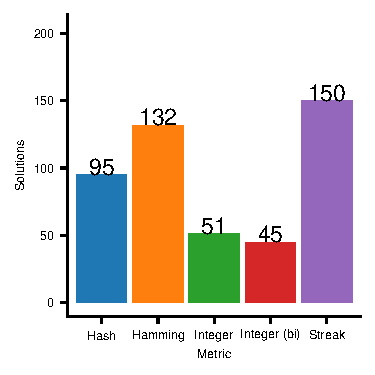
\includegraphics[width=0.75\linewidth]{img/gp_results/panel-dst-sols.pdf}%
\caption{
Numbers of replicates out of 200 that produced a complete solution to the directional-signal task.}
\label{fig:dst-sols}
\end{subfigure}
\begin{subfigure}[b]{\linewidth}
\centering
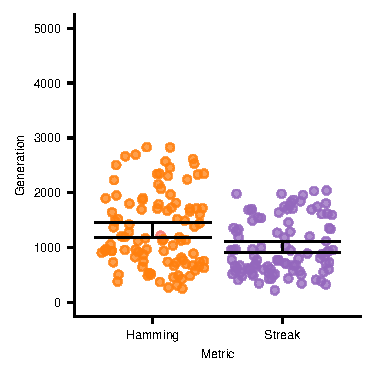
\includegraphics[width=0.75\textwidth]{img/gp_results/panel-dst-times.pdf}%
\caption{
Generations to solution for the first 100 replicates out of 200 to produce a complete solution to the directional-signal task.
Error bars indicate bootstrapped 95\% confidence intervals.
}
\label{fig:dst-times}
\end{subfigure}

\label{fig:gp_results}

\caption{
Evolutionary performance of tag-matching metrics on the directional signals.
All show each metrics' best-performing mutation rate.
}

\label{fig:evo_directional_signal}
\end{figure}

As in the changing-signal task, the directional-signal task requires that programs respond to a sequence of environmental cues. 
In the directional-signal task, however, the correct response to signal depends on the history previously experienced signals.
In the directional-signal task, there are two possible environmental signals --- a `forward signal' and a `backward signal' (each with a distinct tag) ---  and four possible responses.
If a program receives a forward-signal, it should express the next response, and if the program receives, a backward-signal, it should express the previous response.
For example, if response three is currently required, then a subsequent forward signal indicates that response four is required next, while a backward signal would instead indicate that response-two is required next.
Because the appropriate response to both the backward and forward signals change over time, successful programs must regulate which functions these signals trigger (rather than hardcode each response to a particular signal).
SignalGP module tags are more constrained than in the changing-signal task, potentially needing to match to different tagged events (\textit{e.g.}, environmental signals or internally-generated signals) depending on regulatory state well as well as to internal genetic regulation instructions.
Indeed, in other work, we have observed that the directional signal task yields significantly more interconnected regulatory networks than the changing signal task \citep{Lalejini_Moreno_Ofria_2020}.

% Evaluation overview
We evaluate programs on all possible four-signal sequences of forward and backward signals (sixteen total).
For each program, we evaluate each sequence of signals independently, and a program's fitness is equal to its aggregate performance.
Otherwise, evaluation on a single sequence of signals mirrors that of the changing signal task.

% Experiment overview
We used an identical experimental design for the directional-signal task as in the changing signal task. 
However, we evolved programs for 5000 generations (instead of 100) and re-parameterized each metric's tag mutation rate:
%(these data are available in supplemental material \cite{Moreno_Ofria_2020}): 
0.001 for the hamming and hash metrics, 0.002 for the integer and streak metrics, and 0.0001 for the bidirectional Integer Metric. 
Full configuration details for this experiment, including a guide for replication, appears in \href{doi.org/10.17605/OSF.IO/GW5MC}{supplemental material} \cite{Moreno_Ofria_2020}.

% Results
Figure \ref{fig:dst-sols} gives the number of replicates that produced a successful SignalGP program for each tag-matching metric on the directional-signal task.
Again, the hamming and streak metrics performed significantly better than all other metrics (Fisher's exact with a Holm correction for multiple comparisons, $p < 0.0008$). We observed no significant difference in solution count between the hamming and streak metrics, however.
As in the changing-signal task, we assessed whether the streak metric produced solutions in fewer generations than the hamming metric, running 200 new replicates of each condition until 100 replicates produced a solution and recorded the number of generations that elapsed (Figure \ref{fig:dst-times}).
We found that streak metric generally required fewer generations for a solution to evolve than the hamming metric (Wilcoxon rank-sum test, $p < 0.0016$).

As in the changing-signal task, we observed no difference in success between the integer and bidirectional integer metrics on both the changing- and directional-signal tasks.
Again, the hash metric outperformed both the integer metrics ($p < 3\times10^{-5}$).
%Intuitively, the Hash metric maximizes the amount of phenotypic variation (\textit{i.e.}, signal-function relationships) that can be generated by mutating a given genotype --- a single bit flip in a tag is likely to completely re-order which other tags it best matches with.
%The capacity to quickly generate large amounts of phenotypic variation allows evolution to explore a large swaths of the fitness landscape from generation to generation.
%However, this capacity to generate phenotypic variation trades off with tag-matching robustness --- a single mutation may also scramble any established relationships with other tags.
%Further, of each of the metrics we explored, the Hash metric is the most susceptible to mutational meltdowns at high mutation rates.

%[Statement about consistency with expectations based on previous tag-matching experiments].
% - Appears to be consistent with results from graph matching evolution experiment. Needs confirmation, though.
% - Interesting that these two metrics seem to have fairly different geometric properties (because wrap-around vs no wrap-around), but have fairly similar variational properties.
% - For GP problems here, wrap-around vs no wrap around seems to not make a difference.


% TODO - double check that result in analyses
% [Statement about consistency with expectations based on previous tag-matching experiments].
% Seems largely consistent with mean-degree-2 results (for later updates) in graph matching evolution experiment.
% More work to be done, but these data indicate that streak metric can be used for best/consistent performance in GP.

